\documentclass[a4paper,11pt]{report}
\usepackage[utf8x]{inputenc}
\usepackage{a4wide}
\usepackage{fancyhdr}
\usepackage{graphicx}
\usepackage{txfonts}
\usepackage{gantt}
%opening
\title{Automated Chip Tester - System Summary}
\author{Team I}
\author{
 Hornung, Alex \\
 Li, Xiaolong\\
 Progias, Pavlos\\
 Torres, Romel\\
 Zhou, Bo\\
}


\pagestyle{fancy}
\lhead{Automated Chip Tester - Summary}
\chead{}
\rhead{Team I}

\begin{document}

\maketitle

\cfoot{\thepage}

\section*{System Description}
The aim of this project is designing an automated chip tester for the Superchip
Platform\cite{superchip}. These chips contain up to 16 different
designs that must be tested individually (only one at a time); each design
contains an oscillator, thus a measurement of the frequency must be done as
well. Figure \ref{fig:chip_diagram}
shows a diagram of the blocks within the chip to be tested. All the designs
share the input/output ports and each design is selected trough the local power
supply (\emph{individual vdd} on the diagram).
\\


\begin{figure}[htb]
\centering
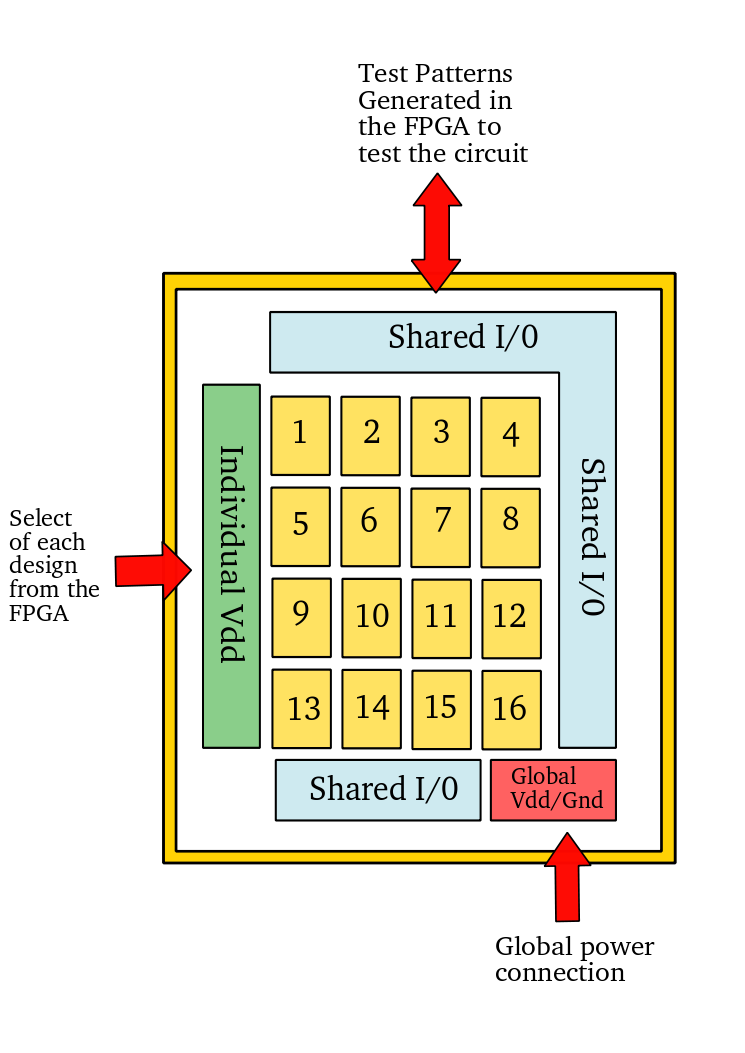
\includegraphics[scale=0.25]{Chip.png}
\caption{Diagram of the chip to be tested, from \cite{superchip}}
\label{fig:chip_diagram}
\end{figure}


The chip tester will be implemented using an Altera DE2-115 Development Board,
featuring an Altera Cyclone IV EP4CE115 and a budget of approximately
\textsterling200
provided by the University of Southampton.
\\


Figure \ref{fig:block_diagram} shows the block diagram of the system to be
designed. An integrated SoPC using a NIos II processor running $\mu C Linux$
will be used as a controller. It will interface with the SDCard and with a host
computer over USB and via Ethernet. Test vectors and expected result vectors
will be loaded via one of the aforementioned methods into fast on-board SRAM.
\\

\begin{figure}[htb]
\centering
%XXX: block diagram is missing SDRAM
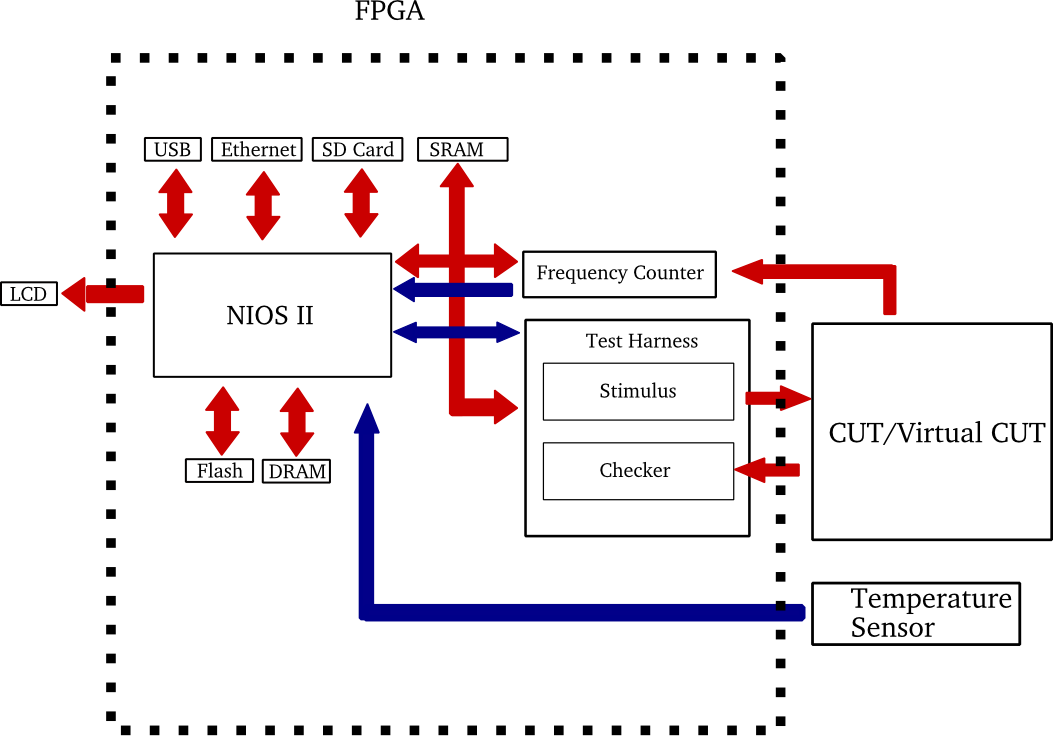
\includegraphics[scale=0.45]{Block_diagram_new.png}
\caption{Block diagram of the initial system on the FPGA}
\label{fig:block_diagram}
\end{figure}


Control is then passed to the Test Harness or runner, which will load one set
of stimuli and expected results at a time and pass them to the stimulus
generator and results checker. Input and output of the stimulus generator and
results checker will be synchronized with the external clock provided by the
design, which is regenerated locally using a PLL.
\\

The stimulus generator enables the Vdd of a particular design as requested by
the test harness (runner) by outputting a 4-bit binary number to the external
interface board. The interface board has a 4-to-16 decoder, with each line
connected to a switch or transistor that will connect the external Vdd to one
of the designs on the chip under test. The board will also contain a
temperature sensor connected to a simple serial bus to record the temperature
during testing, since this is a significant factor influencing IC performance
and even failure.
\\

The results of the verification of each design is stored back to SRAM including
the actual output of the design under test. Once testing is complete, an
interrupt is raised to the controller, which then reads the results from SRAM
and stores and/or processes them.
\\

Additionally a digital frequency counter will be designed, which will allow
measurement of the external clock frequency of each design.
\\

As extended goal a simple one-channel digital storage oscilloscope will be
developed. This allows for quick troubleshooting and analysis of the clock
signal generated on the chip under test. An 8-bit 250MSps external ADC,
differential amplifier and a passive filter will form the first version of the
analog frontend. Triggering will occur on the sampled data on the FPGA.
\\

If time permits this version will be
refined by replacing the differential amplifier with a programmable gain
amplifier to allow for different voltage ranges, as well as a variable filter to
control the passband and proper external triggering implemented with comparators
in the analog frontend.
\\

The sampled analog data will be stored into the fast on-board SRAM and then
processed and displayed, possibly using a graphics LCD or the VGA output.


\newpage
\section*{Tasks}
\vskip 1.5cm


\begin{gantt}{18}{10}
    \begin{ganttitle}
    \numtitle{1}{1}{10}{1}
    \end{ganttitle}
    \ganttbar{Nios II SoPC + run Linux (A,P,R)}{0}{2}
    \ganttbarcon{SoPC: Test vectors from SDCard (A,P,R)}{2}{2}
    \ganttbar{SoPC: USB, configuration (J,R)}{4}{4}
    \ganttbar{SoPC: Ethernet communication (P,R)}{4}{4}
    \ganttbar{PC Software, database frontend (P,R[,A])}{4}{5}

    \ganttbar{Digital frequency counter (A)}{2}{1}
    \ganttbar{Test Harness + SRAM i/f (A)}{3}{2}
    \ganttbar{Stimulus generator (J,N)}{3}{2}
    \ganttbar{Results Checker (J,N)}{4}{1}

    \ganttmilestone[color=red]{Working Chip Tester}{6}

    \ganttbar{Ext. Board design (J,N)}{1}{1}
    \ganttbarcon{Ext. Board PCB Layout + Fab. (J,N)}{2}{2}
    \ganttbarcon{Ext. Board Revision (A,J,N)}{5}{2}
    \ganttbarcon{Ext. Board Rev. PCB Layout + Fab. (A,J)}{7}{2}

    \ganttcon{4}{12}{5}{15}
    \ganttbar{Basic oscilloscope (A,N)}{5}{2}
    \ganttbarcon{Adv. oscilloscope features(A,N,P)}{7}{3}

    \ganttmilestone[color=red]{Working Oscilloscope}{9}
  \end{gantt}

\vskip 1cm

\begin{table}[h!]
\begin{tabular}{l|l}
 {\bf Abbrev.} & {\bf Name} \\
 \hline
 A & Hornung, Alex \\
 J & Zhou, Bo\\
 N & Li, Xiaolong\\
 P & Progias, Pavlos\\
 R & Torres, Romel\\
\end{tabular}
\end{table}

\bibliographystyle{IEEEtran}

\begin{thebibliography}{1}

\bibitem{superchip}
Wilson, P.R.;   Wilcock, R.;   McNally, I.;   Swabey, M.;, \emph{Innovative
Teaching of IC Design and Manufacture Using the Superchip Platform}\hskip 1em
plus
0.5 em minus 0.4em\relax IEEE Transactions on Education, Vol. 53, Issue 2, pp.
297 - 305


\end{thebibliography}



\end{document}
 